\documentclass[fontsize = 12pt, paper = a4]{scrreprt} 

\setlength{\parindent}{0pt}
\usepackage[english,ngerman]{babel}
\usepackage[utf8]{inputenc} 
\usepackage{enumerate}
\usepackage{amssymb,amsmath}

%------------ Überschriften verkleinern und hochsetzen ----------%

\makeatletter
\renewcommand*\@makechapterhead[1]{%
{\parindent \z@ \raggedright \normalfont
\LARGE\bfseries
\ifnum \c@secnumdepth >\m@ne
\thechapter\space
\fi
#1\par\nobreak
\vskip 20\p@
}} 

% ------------------------ Blattlayout- -------------------------%

\usepackage {geometry}   
\geometry   {left     = 2.5cm,
             right    = 2.5cm, 
             top      = 1.5cm,
             bottom   = 1.5cm,
             includehead, includefoot}
             
% ------------------------ Seitenstil ---------------------------%           

% Umdefinieren von Befehlen zur Vermeidung von Bugs:

\renewcommand*{\chapterpagestyle}{scrheadings} 
\renewcommand*{\chapterheadstartvskip}{\vspace*{-\topskip}}

% Gestaltung der Kopf- und Fußzeile:

\pagenumbering{arabic}
            
\usepackage[automark]{scrpage2}
\automark[chapter]{section}
\pagestyle{scrheadings} 
\ohead[\pagemark]{\pagemark}
\setlength{\footskip}{5mm} 

\clearscrheadfoot
\lohead{Entwurfsdokument}
\rohead{\headmark}
\lofoot{Softwareprojekt TU Ilmenau SS 2013}
\rofoot{\pagemark}

% Kopf- und Fußzeilenlinie:

\setheadsepline{.6pt} % Linie für Kopfzeile
\setfootsepline{.6pt} % Linie für Fußzeile 

% Für Unterstreichungen:

\usepackage[normalem]{ulem}

% Buchstabenglättung am Rand:
  
\usepackage {microtype}  

%-------------------------------------------------------------------%

% Für die Einbindung von Bildern:

\usepackage[pdftex]{graphicx} % .pdf, .png oder .jpg möglich!
\usepackage{rotating}         % Grafiken rotieren

% Nutzung in drei Umgebungen möglich:

% (1) \begin{turn}{Winkel} ...  \end{turn}
% (2) \begin{sideways} ... \end{sideways} 90° im math. pos. Sinn
% (3) \begin{rotate}{Winkel} ... \end{rotate} 
%     ---> 90° im math. pos. Sinn, allerdings keine Platzreservierung 

\usepackage{wrapfig}
%\usepackage{picins}   % Textumflossene Grafiken
\usepackage{subfigure}
\usepackage{floatflt}
\usepackage[justification=centering]{caption}

%-------------------------------------------------------------------%
 
% Packete für Tabellen:

\usepackage{booktabs}
\usepackage{array}    % optional
\usepackage{tabularx} % optional

\usepackage[font=footnotesize,labelfont=bf,singlelinecheck=false,
            format=plain,,justification=justified,indention=0cm]                     {caption} 

\usepackage{setspace}

%----------------  Anfang des Dokuments ------------------%

\begin{document}

%*******************************************************************%

% Entwurf Titelseite:

\titlehead{\begin{center}
\textbf{\Huge Entwurfsdokument}
\end{center}}
		   
\title{Service-Interface \\ für ein Formula-Student-Fahrzeug}

\subtitle{Technische Universität Ilmenau \\
		  Softwareprojekt SS 2013 \\ Gruppe 19}			
		
\author{Christian Boxdörfer \\ Thomas Golda \\ Daniel Häger \\ 
		David Kudlek \\  Tom Porzig \\ Tino Tausch \\ 
		Tobias Zehner \\ Sebastian Zehnter}
		
\date{15.05.2013}	 
	  
\publishers{betreut durch \\ \vspace{1cm} Dr. Heinz-Dietrich Wuttke, TU Ilmenau \\ Oliver Dittrich, fachlicher Betreuer Team StarCraft e.V.}

\maketitle		

%*******************************************************************%

% --------------------- Inhaltsverzeichnis -----------------------%

\begin{spacing}{0.95} 
\tableofcontents
%\setcounter{secnumdepth}{4} % Tiefere Gliederungsebene  
\setcounter{tocdepth}{4} % Anzeige bis Gliederungsstufe 4
%\addtocontents{toc}{\protect\enlargethispage{2\baselineskip}} 
\end{spacing}


\newpage % Seitenumbruch

%--------------------------  Einleitung  ---------------------------%

\chapter{Einleitung}

Diese Software ermöglicht es dem Team StarCraft e.V. Daten von ihrem Formula-Student-Fahrzeug Daten in weicher Echtzeit auszulesen und zu visualisieren. Hierfür werden auf einer dSPACE MicroAutoBox II die Daten zu Blöcken gebündelt, per Ethernetverbindung an einen Embedded-PC gesendet und von diesem per UMTS/GPRS an eine Datenbank gesendet, die Daten der letzten 10 Stunden speichern soll. Die Darstellung erfolgt dann über eine Webseite, die die einzelnen Daten aus der Datenbank ausliest und darstellt. Die Webseite soll sich vor allem durch Übersichtlichkeit und leichte Bedienbarkeit auszeichnen, sowie ein Nutzersystem bereitstellen. Das Projekt ist daher viergeteilt in die Abschnitte MicroAutoBox II, Embedded-PC, vServer und Webseite, da in all diesen Abschnitten durch unser Team Arbeiten verrichtet werden. Im Folgenden wird erklärt, wie die Daten zwischen den einzelnen Abschnitten ausgetauscht werden und wie die Abschnitte dies bewerkstelligen.


%------------------------  Randbedingungen  ------------------------%

\chapter{Randbedingungen} 

Hier Text einfügen!

%--------------------------  Grobentwurf  --------------------------%

\chapter{Grobentwurf}

\section{Architekturmuster und Systemzerlegung}

Aufgrund der Komplexität des Systems, was aus einer Vielzahl an unterschiedlichen Plattformen und Funktionen resultiert, lässt sich die Architektur des Systems keinem vorgegebenen Architekturmuster zuordnen. Um dennoch einen Überblick über die einzelnen Systemkomponenten zu ermöglichen, wurden diese in dem folgenden Verteilungsdiagramm modelliert.

\begin{figure}[h]
\centering
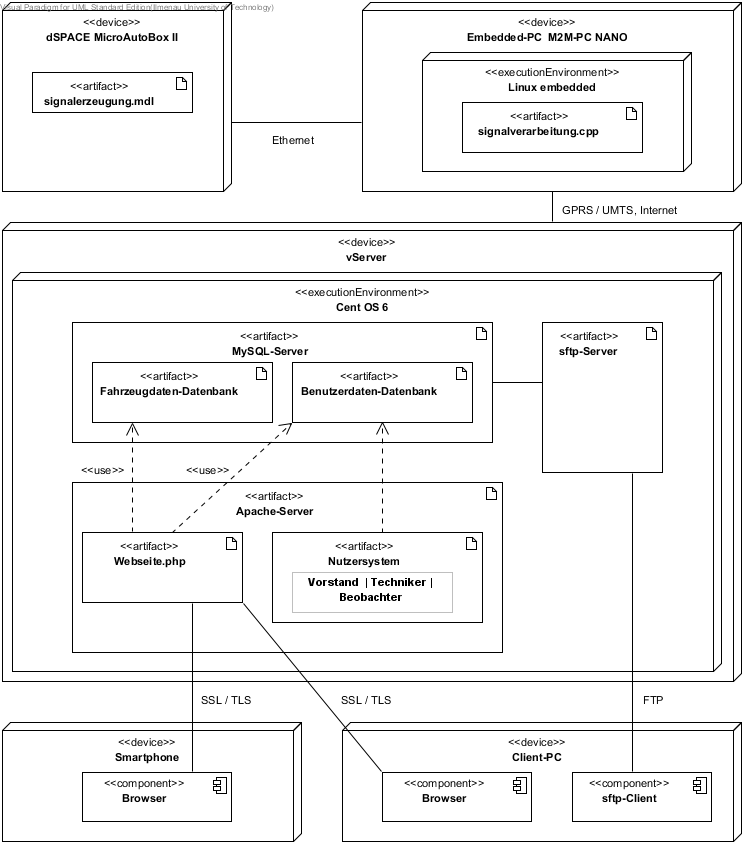
\includegraphics[scale = 0.7]{verteilungsdiagramm.png}
\caption{Gesamtsystem als Verteilungsdiagramm}
\end{figure}

\subsection{dSPACE MicroAutoBox II}

Bei der dSPACE MicroAutoBox II handelt es sich um ein Steuergerät mit Echtzeiteigenschaften, welches fest im Forumla-Student-Fahrzeug verbaut ist und es ermöglicht sämtliche Fahrzeugdaten aus ebendiesem auszulesen. Auf diesem Gerät wird ein Simulink-Modell implementiert, das die als Busarray empfangen Daten entgegennimmt, aufbereitet, enkodiert und über eine UDP-Schnittstelle an einen Embedded-PC überträgt. 

\subsection{Embedded-PC}

Die verwendete MicroAutoBox II sendet die zuvor aufbereiteten Fahrzeugwerte mit Hilfe des auf ebendieser implementierten Simulink-Modells per UDP-Sockets* über einen kabelgebundenen Netzwerkanschluss (LAN) an den Embedded-PC M2M-PC NANO der Firma Adyna. Die Übertragung der Fahrzeugdaten von dem Embedded-PC zu dem virtuellen Server geschieht ebenfalls über UDP-Sockets*. Für die eigentliche Übertragung zum virtuellen Server über UMTS* sind zwei in der Programmiersprache C++ selbst entwickelten Programme - das Server-Programm und das Client-Programm - zuständig. Beide Programme laufen eigenständig auf dem Embedded-PC und werden automatisch beim Systemstart ausgeführt. Ein von der eigentlichen Übertragung ausgeschlossenes und selbst entwickeltes Programm [namens AAAA] garantiert das Ausführen beider Programme und startet die Programme bei einem auftretenden Absturz oder schwerwiegenden Fehler neu. Dabei wird während des Vorgangs das Server-Programm jedem UDP-Packet des Datenstroms* ein Zeitstempel* hinzugefügt, wobei später ankommende Packete ignoriert und erst nach dessen Fertigstellung ein neues Packet behandelt werden \textbf{(Klären?)}. Der hinzugefügte Zeitstempel beinhaltet die Systemzeit des Embedded-PC zum Zeitpunkt des Hinzufügens und dient dazu, die Aktualität der Daten bei dem Eintreffen auf dem virtuellen Server festzustellen. Anschließend leitet das Programm die Daten an das Client-Programm weiter, welches die empfangenen Daten über eine mobile Breitbandverbindung mittels UDP-Sockets an den virtuellen Server weiterleitet. 		


\subsection{Virtueller Server}

Der virtuelle Server wird vom den Provider 1\&1 bereitgestellt und ist jederzeit über eine feste IP* erreichbar. Darauf wird eine Software implementiert, die eingehende Pakete an einem bestimmten Port entgegennimmt, deren Nutzdaten dekodiert, validiert und in eine auf dem virtuellen Server laufende MySQL-Datenbank schreibt. 

\subsection{Webseite}

Die Webseite übernimmt im Rahmen dieses Systems die Aufgaben der grafischen Benutzeroberfläche. Sie besitzt zwei Kernaufgaben: das Darstellen der Fahrzeugdaten, die sich in einer Datenbank auf dem Webserver befinden und das Vermeiden von Zugriffen unbefugter Personen auf eben diese Daten. Dies wird durch ein Benutzersystem erreicht, welches nur ausgewählten Personen ermöglicht an die Informationen der Datenbank zu kommen und sich diese somit darstellen oder exportieren zu lassen.

\subsection{Datenbanken}

\subsubsection{Benutzerdaten-Datenbank}

\subsubsection{Fahrzeugdaten-Datenbank}




%------------------Feiner Rotz-----------------------------------------

\section{Simulink-Modell}
\subsection{Verwendete Blöcke}

Um den Einstieg in unsere im folgenden aufgeführte Modellausschnitte  zu erleichtern, werden im Verlauf dieses Abschnittes alle zur Erstellung des Simulink-Modells für die dSPACE MicroAutoBox II verwendeten Blöcke vorgestellt und ihre Funktionsweise kurz erläutert.

\subsubsection{Sources}
\begin{itemize}

\begin{figure}[h]
  \centering
\begin{minipage}[b]{2.5cm}
    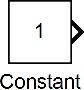
\includegraphics[scale = 0.6]{constant}
    \caption{Constant-Block \label{Constant-Block }}
  \end{minipage}
\hspace*{3cm}  
  \begin{minipage}[b]{5 cm}
    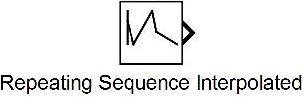
\includegraphics[scale = 0.6]{rsip}
    \caption{Repeating Sequence Interpolated - Block \label{Repeating Sequence Interpolated - Block}}
  \end{minipage}
\end{figure}

\item[1)] \textit{Constant-Block}

%\pichskip{3em}
%\piccaption{Constant-Block \label{Constant-Block}}
%\parpic[r]{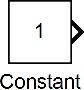
\includegraphics[height = 1.5cm]{constant}}

Der Constant-Block ermöglicht die Generierung eines reellen oder komplexen konstanten Wertes. Je nach Modifikation der Einstellungen 
des Blocks wird es zudem ermöglicht, neben einem konstanten Skalar einen konstanten Vektor oder eine konstante Matrix als Eingangssignal bereitzustellen. Als Datentypen für das Eingangssignal stehen die unter X.Y. aufgeführten Datentypen zur Verfügung.

\item[2)] \textit{"`Repeating-Sequence-Interpolated" \ - Block}

Im Gegensatz zum Costant-Block ermöglicht dieser Block die Erzeugung eines individuellen, sich periodisch wiederholenden und kontinuierlichen Signals mittels einer Interpolation anhand zuvor selbst definierter diskreter Zeit- und Funktionswerte, welche in zwei Vektoren gleicher Länge gespeichert sind.

\end{itemize}

%\newpage

\subsubsection{Ports \& Subsystems}

\begin{itemize}

\begin{figure}[h]
  \centering
  \begin{minipage}[b]{2.5 cm}
    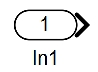
\includegraphics[scale = 0.6]{inport}
    \caption{Inport-Block \label{Inport}}
  \end{minipage}
  \hfill
  \begin{minipage}[b]{2.5 cm}
    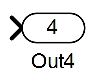
\includegraphics[scale = 0.6]{outport}
    \caption{Outport-Block \label{Outport}}
  \end{minipage}
  \hfill
  \begin{minipage}[b]{3.5 cm}
    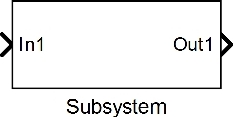
\includegraphics[scale = 0.5]{subsystem}
    \caption{Subsystem \label{Subsystem}}
  \end{minipage}  
\end{figure}


\item[1)] \textit{Inport-Block}

Dieser Block hat in unserem Modell die Aufgabe, die zuvor festgelegten Eingangssignale des Subsystems auf der Modellebene des Subsystems selbst zu repräsentieren. Darüber hinaus mit ist es in der Top-Level-Ebene des Systems mit diesem Block auch möglich, externe Eingangssignale aus dem Arbeitsbereich für das Modell bereitzustellen. 

\item[2)] \textit{Outport-Block}

Die Aufgabe des Outport-Blockes ist es, eine Verknüpfung vom aktuellen System zu einem Zielsystem außerhalb der Modellebene herzustellen.

\item[3)] \textit{Subsystem}

Innerhalb eines Subsystems können verschiedene Blöcke zusammengefasst werden, was eine Strukturierung und Gliederung der Signalflüsse erleichtert und zudem eine deutlich übersichtlichere Darstellung des Modells zur Folge hat. Weiterhin ist es auch möglich, mehrere Subsysteme in einem Subsystem zusammenzufassen, um eine beliebige Tiefe innerhalb der Hierarchie eines Modells zu realisieren. 

%\newpage  

\end{itemize}

\subsubsection{Signal Routing}

\begin{itemize}

\begin{figure}[h]
\centering
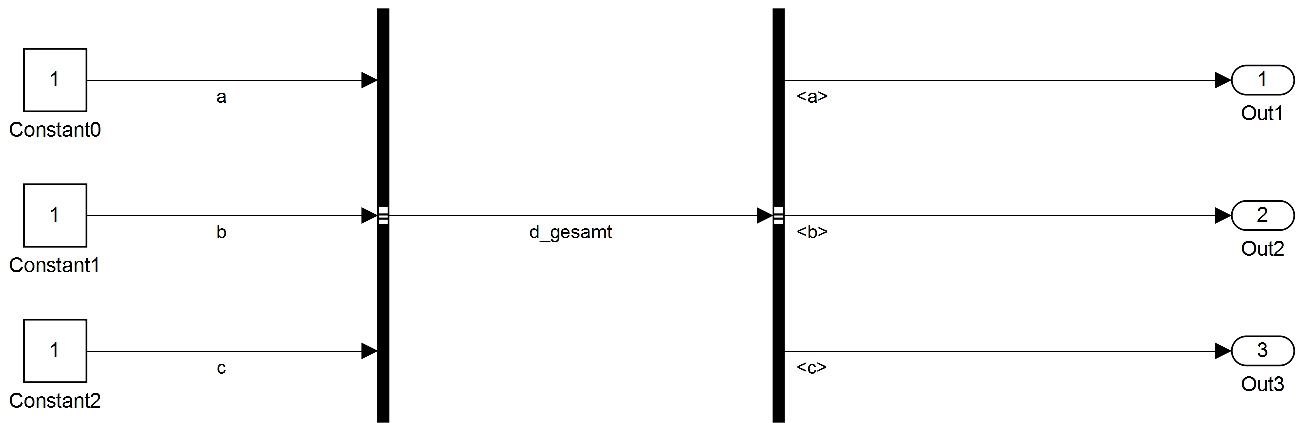
\includegraphics[scale = 0.45]{bus_gesamt}
\caption{Bussystem bestehend aus einem Bus Creator (l.) und einem Bus Selector (r.)}
\end{figure}


\item[1)] \textit{Bus Creator}

Mit Hilfe eines solchen Bus Creators wird es ermöglicht, mehrere Signale (a, b, c) zu einem Gesamtsignal (d\_gesamt) zu bündeln.

\item[2)] \textit{Bus Selector}

Umgekehrt erlaubt es der Bus Selector, aus einem Gesamtsignal wieder einzelne Signale zu selektieren und diese gesondert weiterzuleiten. So wird wie in Abb. X.Y. dargestellt wieder aus dem Gesamtsignal d\_gesamt die Signale a, b und c herausgeführt.

\end{itemize}

\subsubsection{Signal Attributes}

\begin{itemize}

\begin{figure}[h]
  \centering
\begin{minipage}[b]{2.5cm}
    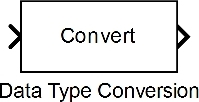
\includegraphics[scale = 0.5]{convert}
    \caption{Convert-Block \label{Convert-Block}}
  \end{minipage}
\hspace*{3cm}  
  \begin{minipage}[b]{5 cm}
    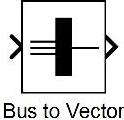
\includegraphics[scale = 0.5]{bustovector}
    \caption{Bus to Vector - Block \label{Bus to Vector - Block}}
  \end{minipage}
\end{figure}

\item[1)] \textit{Convert-Block}

Mit dem Convert-Block können verschiedene Anforderungen realisiert werden:

\begin{itemize}
\item Konvertierung eines Signals bzw. eines Signalvektors in einen anderen Datentyp, hierbei kann die Art der Rundung selbst festgelegt werden.

\item Umbenennung eines Signals bzw. eines Signalvektors. \\
Dies hat den Zweck, dass man nach dem Convert-Block unabhängig vom  angelegten Eingangssignal mit einem festen Datentyp und einem fest vergebenem Variablennamen in anderen Systemen bzw. auf anderen Plattformen arbeiten kann.  

\end{itemize} 

\item[2)] \textit{"`Bus to Vector"\ - Block}

Dieser Block konvertiert ein virtuelles Bussignal in ein Vektorsignal. Hierbei ist es erforderlich, dass alle am zu konvertierenden Bus anliegenden Signale im Datentyp, Signaltyp und im gewählten Sampling-Verfahren übereinstimmen.

\end{itemize}

\subsubsection{Sinks}

\begin{itemize}

\begin{figure}[h]
  \centering
  \begin{minipage}[b]{2.75 cm}
    
\includegraphics[scale = 0.6]{terminator}
    \caption{Terminator-Block \label{Terminator-Block}}
  \end{minipage}
  \hfill
  \begin{minipage}[b]{2.5 cm}
    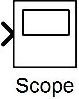
\includegraphics[scale = 0.6]{scope}
    \caption{Scope \label{Scope}}
  \end{minipage}
  \hfill
  \begin{minipage}[b]{3.5 cm}
    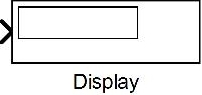
\includegraphics[scale = 0.6]{display}
    \caption{Display \label{Display}}
  \end{minipage}  
\end{figure}


\item[1)] \textit{Terminator}

Der Terminator dient dazu, die Signale, deren Ausgänge nicht mit Blöcken o.ä. verbunden sind, abzuschließen. 

\item[2)] \textit{Scope}

Der Scope-Block stellt den Signalverlauf eines Signals über der Simulationszeit dar, weswegen er sich hervorragend dafür eignet ein erstelltes Modell auf dessen Korrektheit zu überprüfen.

\item[3)] \textit{Display}

Der Display-Block zeigt den konkreten Wert eines Eingangssignals an. Um die Anzeige des Displays anzupassen, kann der Entwickler über die Einstellungen der Format-Parameter Einfluss darauf nehmen.  

\end{itemize}

\subsubsection{Math Operations}


\begin{itemize}

\item[1)] \textit{Gain-Block}

Der Gain-Block multipliziert das Eingangssignal mit einer selbst gewählten Konstante, wobei das Eingangssignal selbst ein Skalar, ein Vektor oder eine Matrix sein kann.


\end{itemize}

\subsubsection{dSPACE-Blöcke}

Im Folgenden sollen nun diejenigen Blöcke vorgestellt werden, welche speziell für eine Verwendung mit der MicroAutoBox II konzipiert wurden und u.a. für eine Kommunikation ebendieser mit dem Embedded-PC unerlässlich sind. 

\begin{itemize}

\item[1)] \textit{Encode32-Block}

\item[2)] \textit{"`UDP Send" \ - Block} 

\end{itemize}

\subsection{Signalgenerator}

Das Modell, welches auf der dSPACE MicroAutoBox II implementiert wird, besitzt zwei Subsysteme - den Signalgenerator und den Signalkollektor. Der Signalgenerator hat hierbei die Aufgabe, auf der MicroAutoBox II die für einen Systemtest benötigten Testsignale zu generieren, welche anschließend zum Embedded-PC via UDP-Schnittstelle gelangen und daraufhin per GPRS / UMTS an einen vServer gesendet werden. Dieses Subsystem wird jedoch nach einem erfolgreichen Test des Service-Interfaces durch ein Subsystem von Team Starcraft e.V. ersetzt, welches im Stande ist die im Formula-Student-Fahrzeug verbauten Komponenten anzusprechen und somit im Unterschied zu dem aktuell verwendeten Signalgenerator statt künstlich erzeugter Daten die realen Daten auszulesen und an den Signalkollektor weiterzuleiten.   

\subsubsection{Struktur des Subsystems}

Um ein hohes Maß an Übersichtlichkeit und Modularität zu gewährleisten, wird an den Vorgaben von Team StarCraft e.V. orientierend das Subsystem des Signalgenerators nochmals in einzelne Subsysteme unterteilt, die die verschieden Kategorien der jeweiligen Fahrzeugdaten repräsentieren. 

\begin{figure}[h]
\centering
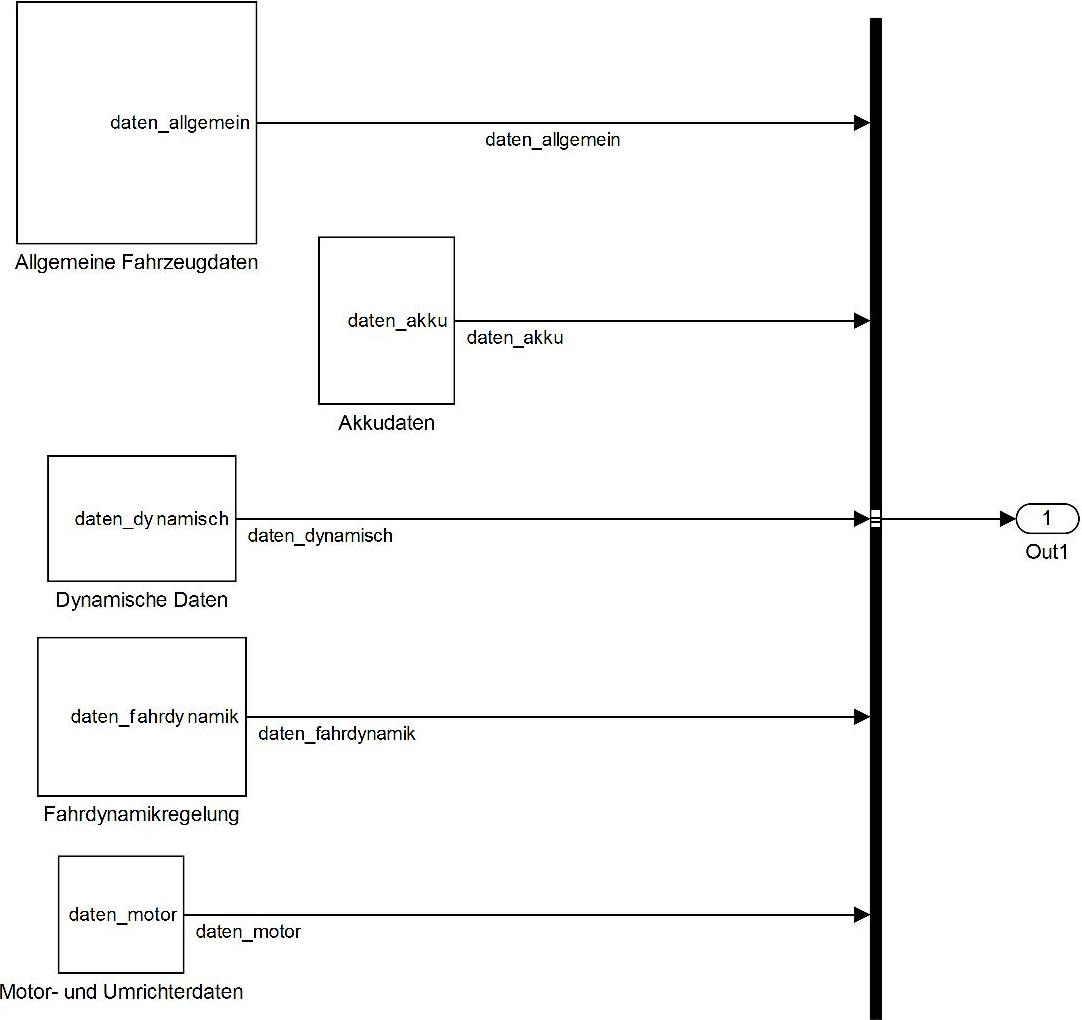
\includegraphics[scale = 0.8]{signalgen}
\caption{Subsysteme des Signalgenerators nach den Kategorien der Fahrzeugdaten}
\end{figure}

Innerhalb dieser Subsysteme findet nun - ohne Beschränkung der Allgemeinheit am Subsystem "`Daten Allgemein"\ erläutert - die Signalerzeugung (Geschwindigkeit, Gesamtspannung des Akkus und der Fahrzeugzeit) statt, wobei wie in X.Y dargestellt die Signalerzeugung mehrere Signale der gleichen "`Signalgruppe"\ wiederum zu Subsystemen (Notausfunktionen, Temperaturen und Gaswerte)  innerhalb des Subsystems "`Allgemeine Daten"\ zusammengefasst werden. Die eigentliche Erzeugung der Signale wird wie in Abbildung X.Y. gezeigt mittels Blöcken aus der Kategorie "`Sources" (s. X.Y) realisiert. Hierbei wird je nach Input entweder ein Constant-Block mit dem Datentyp \textit{boolean} zur Realisierung von Schaltern etc. (s. Notausfunktionen)oder ein Repeating Sequence Interpolated (RSI) - Block mit dem Datentyp \textit{single} zur Modellierung der restlichen Fahrzeugkomponenten verwendet (s. Gaswerte). Der Datentyp \textit{single} wurde deshalb gewählt, um auch wie von Team StarCraft e.V. gefordert als Input Werte mit mehreren Nachkommastellen realisieren zu können. Die auf analoge Weise zu X.Y mit Constant- oder RSI-Blöcken erzeugten 386 Input-Signale werden schließlich im Umkehrschluss zur obigen Beschreibung über mehrere Bussysteme und Subsysteme zu einem Busarray im Signalgenerator zusammengefasst, welcher nunmehr dieses an den Signalkollektor übergibt.   

%\newpage



\begin{figure}[h]
\centering
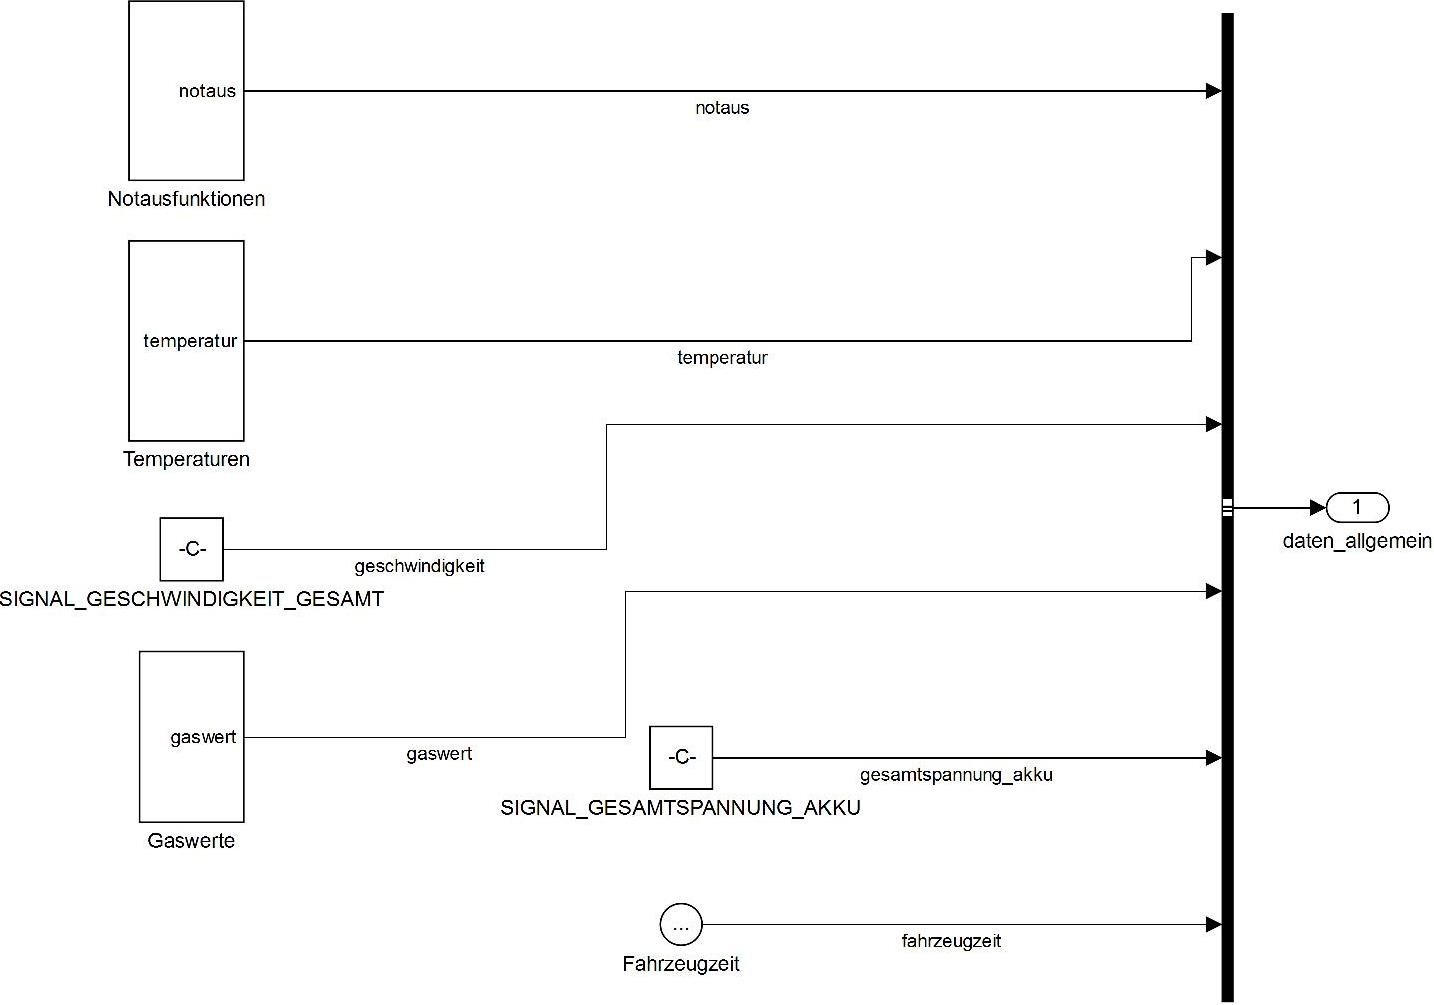
\includegraphics[scale = 0.65]{suballgemein}
\caption{Subsystem "`Allgemeine Daten"\ im Signalgenerator}
\end{figure}
  
\begin{figure}[h]
\centering
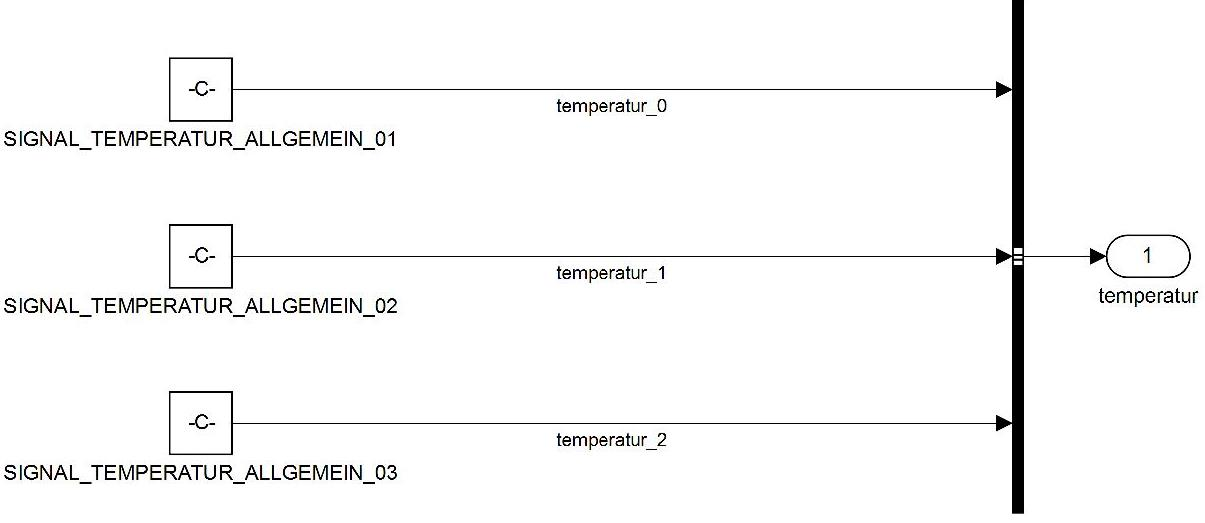
\includegraphics[scale = 0.65]{subsubtemp}
\caption{Signalerzeugung im Subsystem "'Temperaturen"}
\end{figure}


\subsubsection{Config-Datei "`signalgenerator\_microautobox.m" }

Um eine mögliche Änderung der Testsignale zu vereinfachen und eine übersichtliche Darstellung aller Testsignale zu realisieren, sorgt eine Konfigurationsdatei in Matlab für die Spezifizierung der Testsignale des Simulink-Modells. Die in dem *.m-File aufgeführten Parameter für die Zeit- und Funktionsvektoren dienen als Referenz für die signalerzeugenden Blöcke, welche über den Workspace von Matlab auf diese nach dem Ausführen der Datei zugreifen können (s. Abb. X.Y). Hierbei sollte jedoch beachtet werden, dass vor dem Compilieren des Simulink-Modells und der Implementierung ebendiesem auf der MicroAutoBox II einmalig das *.m-File ausgeführt werden muss. Demzufolge muss auch nach dem Ändern von Parametern die Datei neu ausgeführt werden, damit bei einer erneuten Implementierung des Simulink-Modells die geänderten Parameter korrekt übernommen werden können. Zudem wurde auch um die Benennung der Parameter im *.m-File zu standardisieren jeder Funktionsvektor mit dem Präfix "`SIGNAL\_"\ und jeder Zeitvektor mit dem Präfix "`TIME\_"\ versehen. 

\begin{figure}[h]
\centering
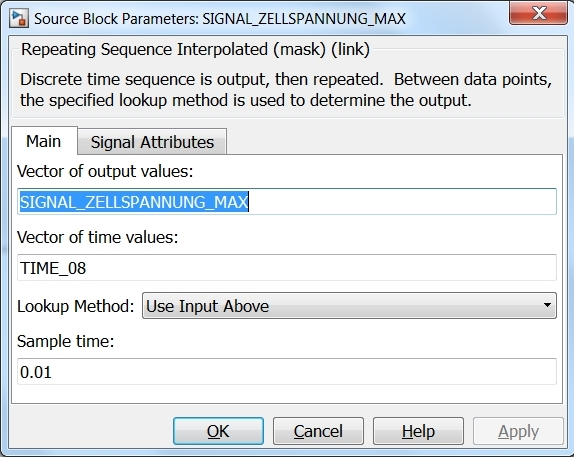
\includegraphics[scale = 0.75]{referenz}
\caption{Referenzierung im RSI-Block}
\end{figure}


\subsection{Signalkollektor}

Der Signalkollektor stellt wie bereits erwähnt das zweite große Subsystem innerhalb des Simulink-Modells dar. Er hat die Aufgabe den vom Subsystem "`Signalgenerator"\ (s. X.Y) oder von einem späteren Subsystem von Team StarCraft e.V. erhaltenen Busarray wieder in die einzelnen Signale zu unterteilen, ggf. geeignet aufzubereiten und diese dann eine UDP-Schnittstelle innerhalb des Subsystems weiterzuleiten, welche die erzeugten Testsignale bzw. Testdaten an den Embedded-PC sendet.  

\subsubsection{Struktur des Subsystems}

Das Subsystem selbst besitzt die folgende innere Struktur: \\
In einem ersten Schritt wird das Busarray wieder in den Kategorien A) - E) der Fahrzeugdaten entsprechenden Signalgruppen aufgeteilt und den fünf Subsystemen (vgl. Abb. X.Y) zugeführt. Dort werden die nunmehr fünf Busarrays wieder über mehrere Busselektoren und Subsysteme hinweg in die 368 einzelnen Signale aufgelöst, welche somit einzeln aufbereitet werden können (s. Abb. X.Y). Während der Aufbereitung der Signale werden die folgenden Schritte durchgeführt:

\begin{figure}[h]
\centering
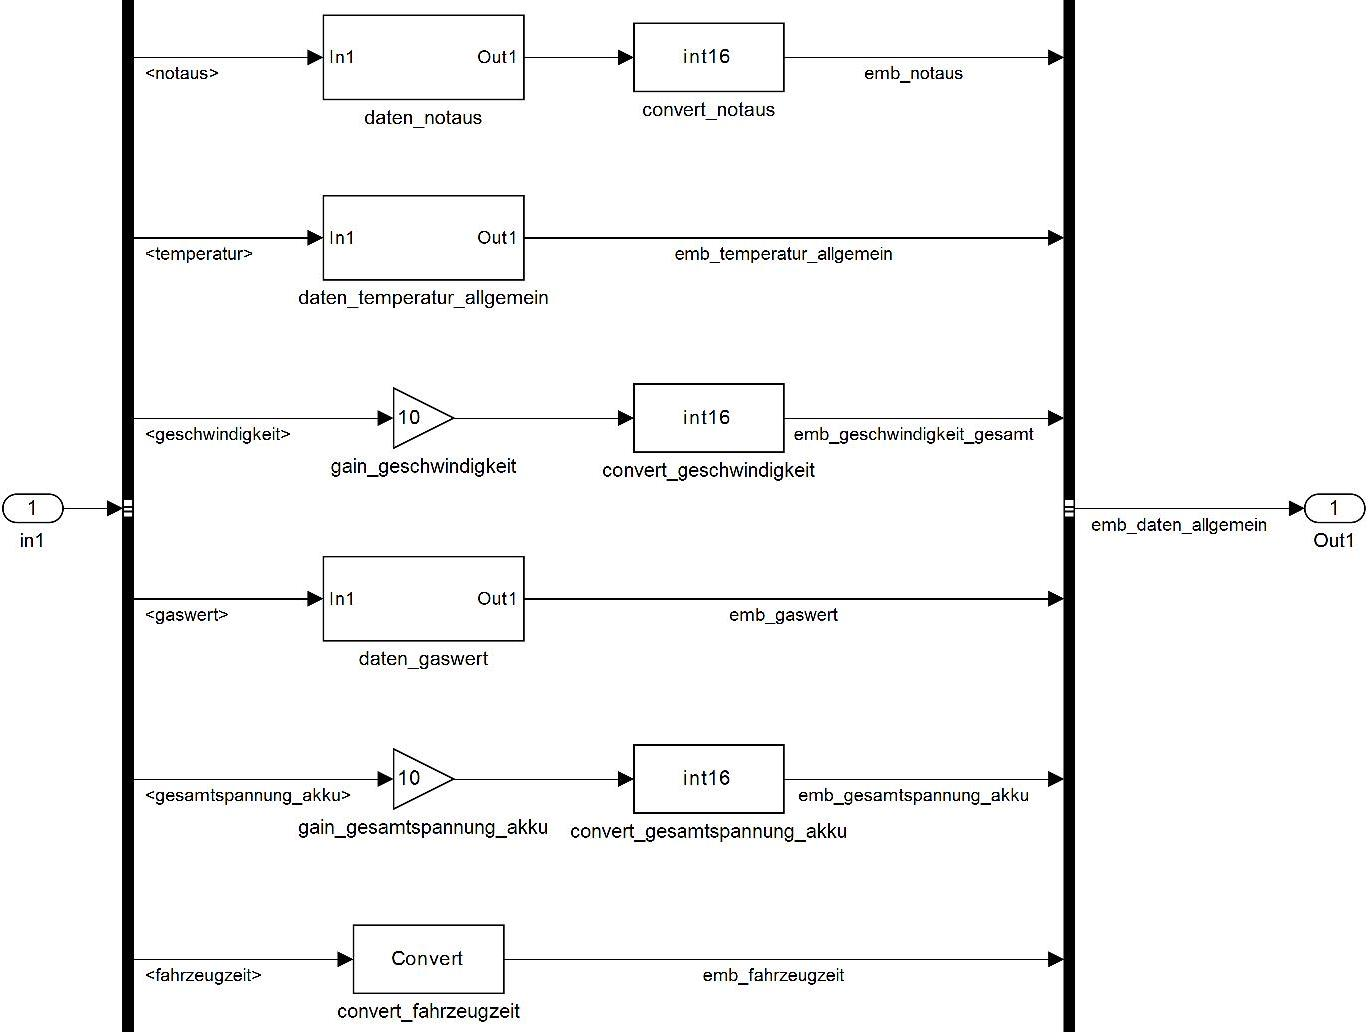
\includegraphics[scale = 0.70]{collallgemein}
\caption{Signalaufbereitung im Subsystem "`daten\_allgemein"}
\end{figure} 


\begin{itemize}

\item[1)] \textit{Verstärkung der Signale}

Abhängig von der Anzahl der Nachkommastellen des Testsignals $n\ mit\ n>0$ wird dieses nun durch einen Gain-Block (s. X.Y) mit dem Faktor $10^n$ multipliziert, um für den aktuellen Wert des Testsignals jeweils einen ganzzahligen Wert zu erhalten, was zur Vereinheitlichung der zu übertragenden Daten beiträgt.

\item[2)] \textit{Konvertierung der Datentypen}

Die nunmehr ganzzahligen Werte werden von ihren Datentypen \textit{boolean} oder \textit{single} nun einheitlich mittels eines Convert-Blocks (s. X.Y) in den Datentyp \textit{int16} konvertiert, wodurch somit alle Signale den gleichen Datentyp aufweisen.  

\item[3)] \textit{Umbenennung der Variablennamen}

Mit dem Convert-Block ist es zudem möglich, dem Ausgangssignal unabhängig vom Eingangssignal einen festen bzw. neuen Variablennamen zu vergeben. Dies ist insofern nützlich, da bei einem möglichen Zugriff auf die Daten bzw. die Variablen durch den Embedded-PC diese immer die gleichen Variablennamen besitzen, unabhängig davon ob der Signalgenerator durch das Subsystem von Team StarCraft e.V. ersetzt wurde oder nicht.

\end{itemize}  

Nachdem die Daten anhand der obigen Schritte aufbereitet wurden, werden dieser erneut durch mehrere Bus Creator und Subsysteme auf einem zentralen Bus Creator zu einem Busarray gebündelt und auf einen Bus to Vector - Block (s. X.Y.) gegeben, welcher das Busarray in einen Vektor umwandelt. Anschließend wird dieser Vektor einem Enkoder (s. X.Y) zugeführt.

\subsection{Enkoder-Block}

Der Enkoder-Block basiert auf einer sFunction die von dSPACE implementiert wurde. Diese konvertiert einen Eingangsvektor in einen Datenstrom mit dem Datentyp \textit{unit32}.

\subsection{UDP-Schnittstelle}

Die UDP-Schnittstelle wird mithilfe zweier Simulink-Blöcke realisiert. Einer ??? 

\section{Embedded-PC}

\subsection{Empfangen der Fahrzeugdaten}

Der Embedded-PC lauscht an einem fest definierten Port nach Paketen welche zuvor von der MicroAutoBox II...  

\subsection{Hinzufügen eines Zeitstempels}

\subsection{Senden der Fahrzeugdaten}


\section{Virtueller Server}


\section{Webseite}

Anhand des nachfolgenden Diagramms soll das Verhalten der Webseite exemplarisch dargestellt werden. Ein registrierter Benutzer ruft in einem Webbrowser die Seite des Service Interfaces auf und loggt sich anschließend über das ihm angezeigte Formular im System ein. Anschließend wird er auf die Seite der allgemeinen Fahrzeugdaten weitergeleitet. Über das Menü steht ihm die Auswahl frei, sich die nach unterschiedlichen Kategorien sortierten Fahrzeugdaten anzeigen zu lassen. Am Beispiel der Akkudaten ruft der Nutzer im Menü über einen Klick auf den Reiter 'Akkudaten' die Seite akkudaten.php auf. Dieses PHP-Skript öffnet eine MySQL-Verbindung und führt nach einem erfolgreichen Verbindungsaufbau eine MySQL-Anfrage aus, die die aktuellsten Akkudaten aus der Fahrzeugdatenbank ermittelt und schließt die Verbindung anschließend wieder. Diese ermittelten Daten werden nun auf unterschiedlichster Art und Weise auf der Webseite dargestellt, sei es nun zum Beispiel als Tabelle oder als einzeln hervorgehobene und gekennzeichnete Sonderinformationen.
Ein JavaScript, welches gleichzeitig im Hintergrund läuft, sorgt dafür, dass die Daten alle $1000 ms$ aktualisiert werden ohne die komplette Seite vollständig neu zu laden. Dabei - und unter Berufung auf die weichen Echtzeitanforderungen - wird die Aktualisierung mittels Timeout realisiert. Anstelle den Server alle $1000 ms$ aufzufordern neue Daten zu schicken, wird nach dem Erhalt der Daten $1000 ms$ gewartet bis eine neue Anfrage gestartet wird. Dies hat zum Vorteil, dass der Server nicht unnötig belastet wird.
Der Benutzer hat jederzeit die Möglichkeit durch die Auswahl eines anderen Reiters im Menü, sich andere Fahrzeugdaten darstellen zu lassen. Das Verhalten läuft analog ab. Vor dem Verlassen wird der Benutzer angehalten sich auszuloggen und seine aktuelle Sitzung somit zu beenden.

\subsection{Registrierung}

Durch das Aufrufen der Seite des TeamStarcraft e. V. Teams lässt sich das Service Interface für das Formula Student Fahrzeug erreichen. Der Besucher erhält eine Aufforderung sich einzuloggen. Es können hierbei unterschiedliche Fälle eintreten:

\begin{itemize}

\item \textit{Fall 1: Der Besucher ist noch nicht registriert.} \\
Sollte er sich noch nicht registriert haben, kann er dies über einen Klick auf einen "`Hier registrieren"\ - Button tun. Der Besucher wird auf eine neue Seite weitergeleitet, die ihm mehrere Formularfelder zur Verfügung stellt. Neben dem Namen (Vor- und Nachname), wird er noch aufgefordert seine Emailadresse und ein Password eingeben. Das eingegebene Passwort muss aus mindestens 6 Zeichen (erlaubt sind Buchstaben in Groß- und /oder Kleinschreibung sowie Ziffern und Sonderzeichen, wobei von jeder Sorte mindestens eines enthalten sein muss) bestehen und muss einmal wiederholt werden. Anschließend kann der Besucher das Anmeldeformular durch einen Klick auf einen Button abschicken. Entsprechen alle Eingaben den Vorgaben werden die Formulardaten in die Nutzerdatenbank eingetragen, andernfalls wird der Nutzer aufgefordert sich mit anderen Daten zu registrieren. Dabei wird das Passwort in verschlüsselter Form und nicht im Klartext abgespeichert. Es wird zudem der Status des Benutzers auf "`nicht aktiviert"\ gesetzt. Anschließend wird eine Email an den Vorstand generiert, die ihn auf die neue Registrierung im System hinweist. Der Vorstand erhält die Möglichkeit die Daten (mit Ausnahme des Passwortes) der registrierten Nutzer einzusehen und deren Status von "`nicht aktiviert"\ auf "`aktiviert"\ zu setzen oder einzelne Benutzer aus dem System zu löschen. Im Falle der Aktivierung des Accounts generiert das System eine Mail, die es an die eingetragene Emailadresse versendet und den Nutzer über die erfolgreiche Aktivierung seines Accounts hinweist.

\end{itemize}

\subsection{Anmeldung}

\begin{itemize}

\item \textit{Fall 2: Der Benutzer ist bereits angemeldet.} \\ 
Zum Anmelden im System ruft der Nutzer die Login-Seite auf und wird anschließend aufgefordert seine Emailadresse und sein Passwort einzugeben. Durch einen Klick auf den Login-Button werden die eingegebenen Daten mit der Nutzerdatenbank verglichen. Sollte die Konstellation aus Emailadresse und dazugehörigem Passwort in der Nutzerdatenbank nicht entdeckt werden, gibt das System eine Fehlermeldung aus, die den Nutzer darauf hinweist, dass die von ihm eingegebenen Daten inkorrekt sind. Sollte das System hingegen einen passenden Eintrag finden, wird abhängig davon, ob der Nutzer bereits aktiviert ist, entweder eine Fehlermeldung (Fall "nicht aktiviert") ausgegeben, oder der Nutzer auf die Seite der allgemeinen Fahrzeugdaten weitergeleitet (Fall "aktiviert"). Der Nutzer kann nun auf der Seite nach Belieben, aber unter Berücksichtung der ihm gegebenen Rechte, auf der Seite des Service Interfaces navigieren.
Sollte in einer gewissen Zeitspanne keine Aktivität vom Benutzer erkannt werden, wird er automatisch aus dem System ausgeloggt.
Ansonsten steht ihm die Möglichkeit, nach getaner Arbeit, sich über den "`Logout"\ - Button auszuloggen und die Seite zu verlassen.

\end{itemize}

\subsection{Passwort vergessen}

\begin{itemize}

\item \textit{Fall 3: Passwort vergessen} \\
Tritt der Fall ein, dass ein im System registrierter Benutzer sein Passwort vergisst, bietet das Nutzersystem ihm die Möglichkeit, sich ein neues Passwort zu setzen. Nach dem Aufruf der Login-Seite muss der Nutzer hierfür auf den Button "Passwort vergessen" klicken und wird anschließend auf eine Seite weitergeleitet, die ihn auffordert seine Emailadresse einzugeben. Durch die Bestätigung der Emailadresse durch den Benutzer prüft das Nutzersystem im Hintergrund, ob ein Eintrag zu dieser Emailadresse existiert. Falls nicht, wird der Vorgang abgebrochen. Der Benutzer erhält aus Sicherheitsgründen kein Feedback darüber. Sollte ein entsprechender Nutzer existieren, generiert das System einen Token, den es mitsamt eines Aktivierungslinks an die angegeben Emailadresse verschickt. Auf der Aktivierungsseite wird der Nutzer erneut aufgefordert seine Emailadresse und den Token anzugeben. Des Weiteren kann er sich an dieser Stelle eine neues Passwort auswählen (selbe Bedingungen wie bei der erstmaligen Registrierung), welches anschließend das alte Passwort im System überschreibt.

\end{itemize}

\subsection{Benutzerverwaltung}

Der Vorstand besitzt als einziger Nutzer im System die Möglichkeit der Verwaltung aller registrierten Systemnutzer. Hierfür steht ihm neben den Übersichtsseiten für die einzelnen Kategorien an Informationen eine spezielle Seite "Benutzerverwaltung" zur Verfügung. Diese Seite stellt die Daten aller angemeldeten Nutzer dar und gibt Auskunft über deren Status im System, also ob sie bereits aktiviert worden sind oder eine Aktivierung noch aussteht. Gelöschte Benutzer werden nicht angezeigt. Ein Aufruf der Seite der Benutzerverwaltung resultiert in einem Verbindungsaufbau mit der Nutzerdatenbank. Bei erfolgreichem Verbindungsaufbau erfolgt anschließend das Versenden eines MySQL-Query, das als Resultat alle im System befindlichen Nutzer ausgibt. Anschließend wir die MySQL-Verbindung wieder getrennt. Die Ausgabe beinhaltet dabei Informationen wie Vor- und Nachname, Rechtegruppe, Accountstatus und eine Information über den letzten Zeitpunkt einer Aktivität des Nutzers. Mittels verschiedener Buttons erhält der Vorstand die Möglichkeit alle Nutzer komplett zu verwalten, d.h. sie aus dem System zu entfernen, sie nach einer Registrierung zu aktivieren oder abzulehnen (und somit zu löschen) oder ihre Rechtegruppenzugehörigkeit festzulegen / zu ändern. Ist der Vorstand fertig mit der Verwaltung der Nutzer, kann er entweder weiterhin auf der Seite navigieren  und arbeiten oder sich ausloggen und die Seite im Anschluss verlassen.


\section{Datenbanken}

\subsection{Benutzerdaten-Datenbank}

Die Aufgabe der Nutzerdatenbank ist das Aufbewahren aller Informationen der registrierten Benutzer. Sie besteht aus drei Tabellen (s. X.Y), welche im Folgenden erläutert werden sollen:

\begin{figure}[h]
\centering
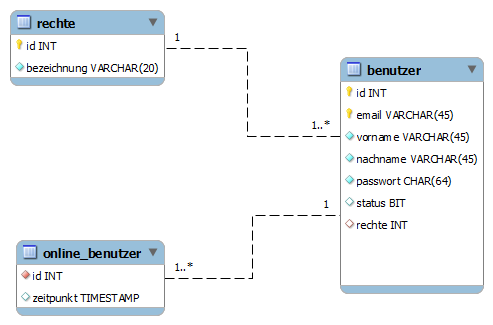
\includegraphics[scale = 0.6]{nutzerdatenbank} 
\caption{Entwurf der Fahrzeugdatenbank}
\end{figure} 

\begin{itemize}
\item[1)] \textit{rechte:} 
In dieser Tabelle befinden sich sämtliche verfügbaren Rechte-Stufen, die sich aus einer eindeutigen ID und einer Bezeichnung in Textform zusammensetzen.

\item[2)] \textit{benutzer:} 
Alle registrierten Nutzer werden in dieser Tabelle gespeichert. Dabei besitzt jeder Nutzer eine eindeutige ID. Diese wird durch automatisches Inkrementieren von der Datenbank erzeugt. Mit der Emailadresse zusammen bilden beide den Primärschlüssel zur eindeutigen Identfikation eines Nutzers. Des Weiteren gehören zu einem Benutzereintrag noch ein Vor- und ein Nachname. Das vom Benutzer bei seiner Registrierung gewählte Passwort wird in gehashter Form als String gespeichert. Ein einzelnes Bit gibt zudem Auskunft darüber, ob der Nutzer bereits vom Vorstand aktiviert wurde und somit Zugang zu den Fahrzeugdaten erhalten hat. Das Feld "rechte" ist Fremdschlüssel zur Tabelle "`rechte"\ und beinhaltet eine der dort befindlichen IDs.

\item[3)] \textit{online\_benutzer:} 
Diese Tabelle speichert Nutzer-IDs und Zeitstempel und gibt somit Auskunft über den Zeitpunkt der letzten Aktivität eines Nutzers.

\end{itemize}

\subsection{Fahrzeugdaten-Datenbank}

Die zweite Datenbank beinhaltet die aus dem Fahrzeug entnommen Daten und bildet gleichzeitig auch die Schnittstelle zur Webseite. Sie besteht aus fünf Tabellen, die jeweils sämtliche Informationen einer Kategorie in sich kapseln (s. Abb. X.Y). Alle Tabellen besitzen über ihre Daten hinaus jeweils noch ein Feld, in dem sich ein Zeitstempel befindet und eines, das für Testzwecke Informationen speichern kann. Anhand des (im Fahrzeug erzeugten) Zeitstempels lassen sich die Datentupel der einzelnen Tabellen einander zuordnen. Im Folgenden werden die Informationen der einzelnen Tabellen erläutert:

\begin{figure}[h]
\centering
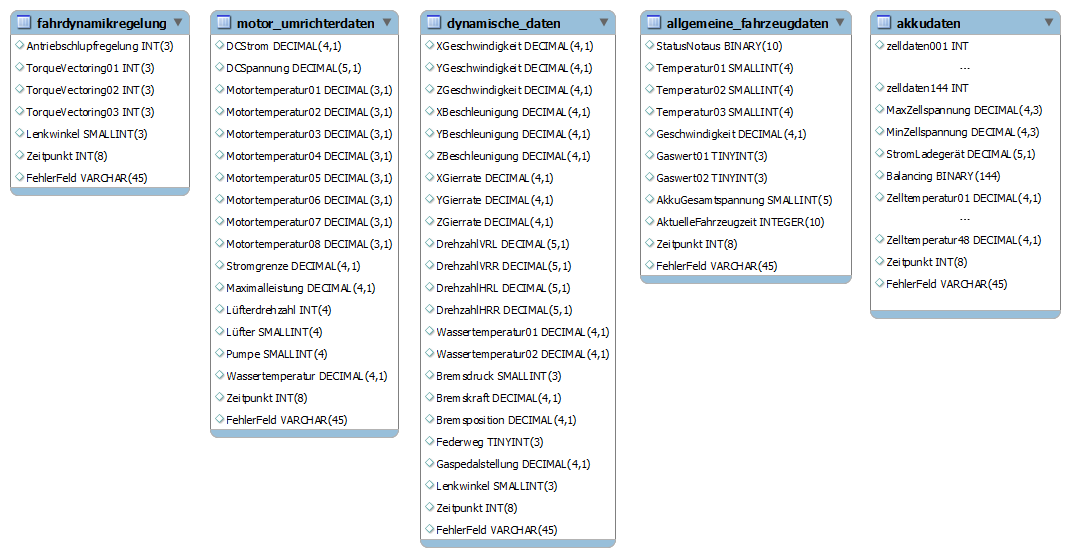
\includegraphics[scale = 0.43]{fahrzeugdatenbank} % Anm: neue Grafik!
\caption{Entwurf der Fahrzeugdatenbank}
\end{figure} 

\begin{itemize}

\item[1)] \textit{fahrdynamikregelung:} 
Diese Tabelle beinhaltet, wie der Name bereits verrät, alle Informationen bezüglich der Fahrdynamikregelung. Sie hält aktuelle Informationen über den Status der Antriebsschlupfregelung, dem Torque-Vectoring in x-, y- und z-Richtung sowie den Lenkwinkel.

\item[2)] \textit{motor\_umrichterdaten:}
Alle Daten, die den Motor und Umrichter betreffen, werden hier gespeichert. Informationen über den aktuell anliegenden Strom oder die aktuell anliegende Spannung sowie die Informationen aller acht Temperatursensoren des Motors lassen sich hier wiederfinden. Ebenso auch Informationen, die die Kühlung des Motors betreffen, wie Lüfterdrehzahlen, Pumpenleistung, Wassertemperatur und eingestellte Stromgrenzen.

\item[3)] \textit{dynamische\_daten:}
Alle Informationen, die die dynamischen Aspekte des Fahrzeugs betreffen, sind hier enthalten. Dies sind beispielsweise die Geschwindigkeiten, Beschleunigungen und Gierraten jeweils in x-, y- und z-Richtung, genau wie die Drehzahlen jedes einzelnen Rads. Desweiteren finden sich hier auch Informationen zu den Bremsen, wie Bremsdruck, -kraft und -position wieder. Auch der Lenkwinkel, der Federweg und die Gaspedalstellung ergänzen das Set der Daten.

\item[4)] \textit{allgemeine\_fahrzeugdaten:} 
Die wichtigsten und allgemeinsten Informationen des Fahrzeugs befinden sich in dieser Tabelle. Neben den wichtigen Informationen wie zum Beispiel den Status der einzelnen Notaus-Schalter des Fahrzeuges, finden sich hier die Werte der drei wichtigsten Temperatursensoren, die aktuelle Fahrgeschwindigkeit, die Gaswerte der beiden Elektromotoren sowie die Gesamtspannung des Akkus und die aktuelle Fahrzeugzeit.

\item[5)] \textit{akkudaten:} Dies ist die letzte und zugleich auch die umfangreichste Tabelle. Hier befinden sich sämtliche Informationen über die im Fahrzeug verbauten Akkus. Neben globaleren Informationen wie die maximale und minimale Zellspannung und dem Strom bzw. der Spannung zum Ladegerät, finden sich die Zelldaten aller 144 Akkuzellen sowie die Temperaturen aller 48 Temperatursensoren wieder. Das Feld "`Balancing"\ gibt darüber hinaus Informationen darüber, ob für die einzelnen Zellen die Balancing-Option aktiviert oder deaktiviert ist.

\end{itemize}


\chapter{Testdrehbuch}




%---------------------------  Glossar  -----------------------------%

\chapter*{Glossar}
\addcontentsline{toc}{chapter}{Glossar}

%----------------------  Abbildungsverzeichnis  --------------------%

%\chapter*{Abbildungsverzeichnis}

\listoffigures

\addcontentsline{toc}{chapter}{Abbildungsverzeichnis}
%
%---------------------------  Anhang  ------------------------------%

\chapter*{Anhang}
\addcontentsline{toc}{chapter}{Anhang}

\appendix

%\textbf{Datentypen in Simulink}
%
%\begin{itemize}
%
%\item xd
%
%\end{itemize}



\end{document}